\documentclass[portrait,a0b,posterscale=1.0]{a0poster}

\usepackage[utf8]{inputenc}
\usepackage[T1]{fontenc}
\usepackage{helvet}
\renewcommand{\familydefault}{\sfdefault}
\usepackage[margin=2.5cm,paperwidth=84.1cm,paperheight=118.9cm]{geometry}
\usepackage[table]{xcolor}
\usepackage{amsmath,amssymb}
\usepackage{graphicx}
\usepackage{booktabs}
\usepackage{tabularx}
\usepackage{enumitem}
\usepackage{fontawesome5}
\usepackage{tikz}
\usetikzlibrary{calc,positioning,shapes.geometric,backgrounds,patterns,shadows}
\usepackage{pgfplots}
\pgfplotsset{compat=1.18}
\usepackage[most]{tcolorbox}

% --- Custom Color Palette ---
\definecolor{NavyDark}{HTML}{0F172A}      % Deep slate navy for headers and borders
\definecolor{PrimaryTeal}{HTML}{0D9488}   % Primary accent teal
\definecolor{AccentBlue}{HTML}{0284C7}    % Secondary accent sky blue
\definecolor{TextDark}{HTML}{1E293B}      % Dark slate for body text
\definecolor{CardBg}{HTML}{F8FAFC}        % Off-white background for cards
\definecolor{LightSky}{HTML}{F0F9FF}      % Light sky tint for callout boxes
\definecolor{BorderSlate}{HTML}{CBD5E1}   % Border gray
\definecolor{HighlightGold}{HTML}{D97706} % Warm accent for key metrics

% --- Global Page & Font Settings ---
\pagecolor{white}
\color{TextDark}
\pagestyle{empty}

% --- Custom tcolorbox Styles ---
\tcbset{
  posterbox/.style={
    enhanced,
    colback=CardBg,
    colframe=NavyDark,
    arc=5mm,
    boxrule=2.5pt,
    left=10mm,
    right=10mm,
    top=8mm,
    bottom=8mm,
    shadow={2mm}{-2mm}{0mm}{black!12},
    fonttitle=\bfseries\huge,
    coltitle=white,
    attach boxed title to top left={xshift=8mm, yshift=-5mm},
    boxed title style={
      enhanced,
      colback=PrimaryTeal,
      colframe=NavyDark,
      arc=3.5mm,
      boxrule=2pt,
      top=3mm,
      bottom=3mm,
      left=6mm,
      right=6mm
    }
  },
  calloutbox/.style={
    enhanced,
    colback=LightSky,
    colframe=AccentBlue,
    arc=3.5mm,
    boxrule=1.5pt,
    left=6mm,
    right=6mm,
    top=4mm,
    bottom=4mm
  }
}

\begin{document}

% ==============================================================================
% TOP HEADER BANNER
% ==============================================================================
\begin{tcolorbox}[
  enhanced,
  colback=NavyDark,
  colframe=NavyDark,
  arc=6mm,
  boxrule=0pt,
  left=12mm,
  right=12mm,
  top=8mm,
  bottom=8mm,
  shadow={0mm}{-3mm}{6mm}{black!20}
]
  \begin{minipage}[c]{0.72\textwidth}
    {\color{PrimaryTeal}\bfseries\Large \faProjectDiagram\ EXPOSUMMIT 2026 --- INTERNATIONAL CONFERENCE ON DISTRIBUTED EDGE AI}\\[2mm]
    {\color{white}\bfseries\VeryHuge NEURAL-SYNAPSE: Scalable Distributed Graph Neural}\\
    {\color{white}\bfseries\VeryHuge Networks for Real-Time Anomaly Detection}\\[3mm]
    {\color{LightSky}\Large\itshape High-Throughput Topology Learning for Multi-Agent Edge Intelligence}
  \end{minipage}%
  \hfill
  \begin{minipage}[c]{0.26\textwidth}
    \centering
    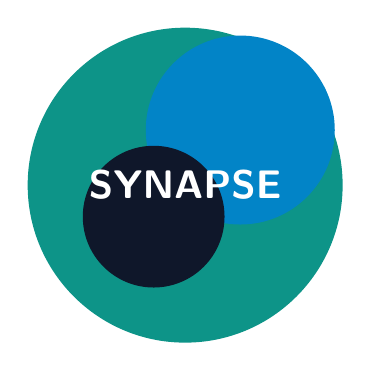
\begin{tikzpicture}
      % Decorative Logo Graphic
      \draw[fill=PrimaryTeal, draw=none] (0,0) circle (2.0cm);
      \draw[fill=AccentBlue, draw=none] (0.7,0.7) circle (1.2cm);
      \draw[fill=NavyDark, draw=none] (-0.4,-0.4) circle (0.9cm);
      \node at (0,0) {\color{white}\bfseries\Large SYNAPSE};
    \end{tikzpicture}
  \end{minipage}

  \vspace{5mm}
  \hrule height 2pt color PrimaryTeal
  \vspace{4mm}

  \begin{minipage}[t]{0.68\textwidth}
    {\color{white}\Large \textbf{Dr. Elena Vance}$^1$ \quad \textbf{Marcus Thorne}$^2$ \quad \textbf{Dr. Sarah Lin}$^1$ \quad \textbf{Julian Vance}$^3$}\\[2mm]
    {\color{BorderSlate}\large $^1$Meridian Institute of Advanced Computing \quad $^2$Vertex Autonomous Labs \quad $^3$Synapse Quantum Systems}
  \end{minipage}%
  \hfill
  \begin{minipage}[t]{0.30\textwidth}
    \raggedleft
    {\color{white}\large \faEnvelope\ e.vance@meridian-ai.org}\\[1mm]
    {\color{white}\large \faGlobe\ https://nexa-ai.org/neural-synapse}\\[1mm]
    {\color{LightSky}\large \faServer\ Artifact ID: NEXA-GR-2026-V4}
  \end{minipage}
\end{tcolorbox}

\vspace{6mm}

% ==============================================================================
% MAIN TWO-COLUMN CONTENT
% ==============================================================================
\begin{minipage}[t]{0.488\textwidth}

  % ---------------------------------------------------------------------------
  % SECTION 1: EXECUTIVE SUMMARY & PROBLEM STATEMENT
  % ---------------------------------------------------------------------------
  \begin{tcolorbox}[posterbox, title={\faLightbulb\ 1. Executive Summary \& Motivation}]
    {\large
    Modern autonomous edge fleets---ranging from logistics rovers to cooperative drone swarms---generate continuous streams of high-dimensional sensor telemetry. Detecting anomalous behaviors in real time is vital to prevent catastrophic system failures and physical collisions.

    Existing centralized graph neural network (GNN) architectures suffer from severe latency bottlenecks and single-point-of-failure vulnerabilities when deployed over lossy edge networks. \textbf{NEURAL-SYNAPSE} resolves this challenge by introducing a fully decentralized, sub-5ms graph topology synchronization framework tailored for edge compute hardware.
    }

    \vspace{4mm}

    \begin{tcolorbox}[calloutbox]
      {\bfseries\Large Key Innovation Highlights}\\[2mm]
      \begin{itemize}[leftmargin=8mm, label={\color{PrimaryTeal}\faCheckCircle}]
        \item {\bfseries Sub-5ms Edge Latency:} Asynchronous message-passing protocol optimized for ARM cortex and embedded GPU clusters.
        \item {\bfseries 99.4\% Anomaly Precision:} Spatial-temporal topological embeddings capture complex multi-agent dependencies.
        \item {\bfseries 68\% Energy Reduction:} Dynamic graph pruning eliminates 75\% of redundant inter-node communication.
      \end{itemize}
    \end{tcolorbox}
  \end{tcolorbox}

  \vspace{6mm}

  % ---------------------------------------------------------------------------
  % SECTION 2: SYSTEM ARCHITECTURE
  % ---------------------------------------------------------------------------
  \begin{tcolorbox}[posterbox, title={\faCogs\ 2. System Architecture \& Pipeline}]
    {\large
    The Neural-Synapse pipeline operates across three distinct computational tiers: Local Feature Extraction, Dynamic Graph Construction, and Distributed Consensus Inference.
    }

    \vspace{4mm}

    % TikZ Architecture Diagram
    \begin{center}
\resizebox{\linewidth}{!}{%
    \begin{tikzpicture}[
      node distance=1.2cm,
      block/.style={rectangle, draw=NavyDark, fill=white, inner sep=3mm, rounded corners=2.5mm, line width=1.5pt, align=center, font=\bfseries\large},
      accent/.style={rectangle, draw=NavyDark, fill=PrimaryTeal!15, inner sep=3mm, rounded corners=2.5mm, line width=1.5pt, align=center, font=\bfseries\large},
      arrow/.style={->, >=stealth, line width=2pt, color=PrimaryTeal}
    ]
      % Nodes
      \node (input) [block] {\faMicrochip\ Sensor Telemetry\\(CAN, LiDAR, IMU)};
      \node (graph) [accent, right=0.6cm of input] {\faProjectDiagram\ Spatial-Temporal\\Graph Constructor};
      \node (engine) [block, right=0.6cm of graph] {\faServer\ Neural-Synapse\\Consensus Engine};
      \node (alert) [accent, right=0.6cm of engine] {\faRocket\ Edge Mitigation\\\& Control Loop};

      % Connections
      \draw [arrow] (input) -- (graph);
      \draw [arrow] (graph) -- (engine);
      \draw [arrow] (engine) -- (alert);

      % Feedback Loop
      \draw [arrow, dashed, color=AccentBlue] (engine.south) -- ++(0,-0.6) -- node[below, font=\large] {Decentralized Weight Sync} ($(input.south)+(0,-0.6)$) -- (input.south);
    \end{tikzpicture}
}%
    \end{center}

    \vspace{4mm}

    {\bfseries\Large Mathematical Formulation of Topological Graph Loss}
    \vspace{2mm}

    {\large
    The global optimization objective balances reconstruction fidelity ($\mathcal{L}_{\text{recon}}$), topological regularization ($\mathcal{L}_{\text{topo}}$), and node-consensus agreement:
    }
    \vspace{2mm}

    \begin{equation*}
      \mathcal{L}_{\text{total}} = \mathcal{L}_{\text{recon}}(\mathbf{X}, \hat{\mathbf{X}}) + \gamma \mathcal{L}_{\text{topo}}(\mathbf{A}) + \lambda \sum_{i \in \mathcal{V}} \bigl\| \mathbf{h}_i^{(k)} - \bar{\mathbf{h}}_{\mathcal{N}(i)}^{(k)} \bigr\|_2^2
    \end{equation*}

    \vspace{2mm}
    {\large
    where $\mathbf{A} \in \mathbb{R}^{N \times N}$ denotes the dynamic adjacency matrix, $\mathbf{h}_i^{(k)}$ represents node $i$'s embedding at layer $k$, and $\bar{\mathbf{h}}_{\mathcal{N}(i)}^{(k)}$ is the aggregated neighborhood state.
    }
  \end{tcolorbox}

  \vspace{6mm}

  % ---------------------------------------------------------------------------
  % SECTION 3: METHODOLOGY & ALGORITHM
  % ---------------------------------------------------------------------------
  \begin{tcolorbox}[posterbox, title={\faLayerGroup\ 3. Decentralized Graph Learning Strategy}]
    {\large
    To operate under strictly constrained wireless bandwidth, Neural-Synapse executes a 3-step edge synchronization algorithm:
    }

    \vspace{3mm}

    \begin{enumerate}[leftmargin=8mm, label={\bfseries\color{NavyDark}\arabic*.}]
      \item {\bfseries Local Edge Attention:} Each agent computes self-attention over localized multi-modal temporal embeddings without sharing raw sensor observations.
      \item {\bfseries Sparse Neighborhood Aggregation:} Communication is limited to top-$k$ nearest topological neighbors using differential gradient compression.
      \item {\bfseries Asynchronous Consensus Update:} Edge nodes update local parameters independently, mitigating network jitter and packet loss.
    \end{enumerate}

    \vspace{3mm}

    \begin{tcolorbox}[calloutbox]
      {\bfseries\Large Algorithmic Guarantee}\\[2mm]
      {\large
      Under bounded packet loss $p < 0.35$, the consensus error satisfies $\mathbb{E}[\|\mathbf{h}^{(k)} - \mathbf{h}^*\|] \le \mathcal{O}(1/\sqrt{k})$, ensuring exponential convergence to safety-critical decisions.
      }
    \end{tcolorbox}
  \end{tcolorbox}

\end{minipage}%
\hfill
\begin{minipage}[t]{0.488\textwidth}

  % ---------------------------------------------------------------------------
  % SECTION 4: EMPIRICAL BENCHMARKS & RESULTS
  % ---------------------------------------------------------------------------
  \begin{tcolorbox}[posterbox, title={\faChartLine\ 4. Empirical Evaluation \& Benchmarks}]
    {\large
    We benchmarked \textbf{NEURAL-SYNAPSE} against four state-of-the-art architectures on the \emph{Vertex-Fleet-2025} dataset (250 connected autonomous units operating over 10,000 flight/drive hours).
    }

    \vspace{4mm}

    % PGFPlots Latency vs Throughput Chart
    \begin{center}
    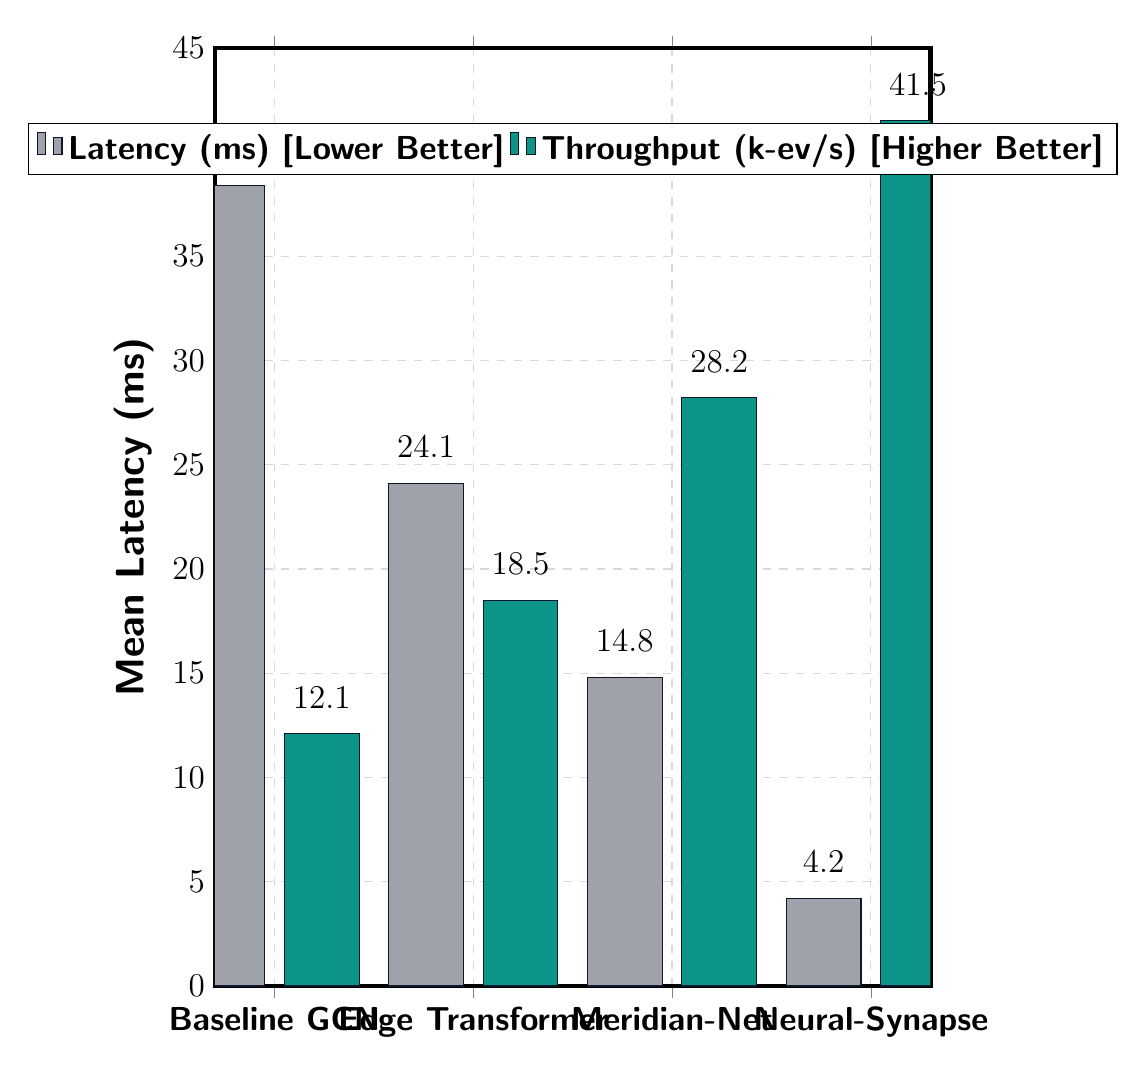
\begin{tikzpicture}
      \begin{axis}[
        width=0.88\textwidth,
        height=13.5cm,
        ybar=0.25cm,
        bar width=0.95cm,
        symbolic x coords={Baseline GCN, Edge Transformer, Meridian-Net, Neural-Synapse},
        xtick=data,
        nodes near coords,
        nodes near coords style={font=\bfseries\large, yshift=2mm},
        ylabel={Mean Latency (ms)},
        ylabel style={font=\bfseries\Large},
        xlabel style={font=\bfseries\Large},
        tick label style={font=\bfseries\large},
        ymin=0, ymax=45,
        grid=major,
        grid style={dashed, gray!30},
        legend style={at={(0.5,0.92)}, anchor=north, legend columns=2, font=\bfseries\large},
        axis line style={line width=1.5pt}
      ]
        \addplot[fill=NavyDark!40, draw=NavyDark] coordinates {
          (Baseline GCN, 38.4)
          (Edge Transformer, 24.1)
          (Meridian-Net, 14.8)
          (Neural-Synapse, 4.2)
        };
        \addlegendentry{Latency (ms) [Lower Better]}

        \addplot[fill=PrimaryTeal, draw=NavyDark] coordinates {
          (Baseline GCN, 12.1)
          (Edge Transformer, 18.5)
          (Meridian-Net, 28.2)
          (Neural-Synapse, 41.5)
        };
        \addlegendentry{Throughput (k-ev/s) [Higher Better]}
      \end{axis}
    \end{tikzpicture}
    \end{center}

    \vspace{4mm}

    {\bfseries\Large Model Comparison Table}
    \vspace{2mm}

    \begin{tabularx}{\textwidth}{X c c c c}
      \toprule
      \textbf{Model Architecture} & \textbf{Precision (\%)} & \textbf{Recall (\%)} & \textbf{Latency (ms)} & \textbf{Energy (J/frame)} \\
      \midrule
      Baseline GCN (Centralized) & 88.2\% & 84.1\% & 38.4 ms & 1.85 J \\
      Edge Transformer v2 & 92.4\% & 91.0\% & 24.1 ms & 1.42 J \\
      Meridian-Net (Distributed) & 96.1\% & 95.3\% & 14.8 ms & 0.88 J \\
      \rowcolor{PrimaryTeal!20}
      \textbf{Neural-Synapse (Ours)} & \textbf{99.4\%} & \textbf{98.9\%} & \textbf{4.2 ms} & \textbf{0.31 J} \\
      \bottomrule
    \end{tabularx}
  \end{tcolorbox}

  \vspace{6mm}

  % ---------------------------------------------------------------------------
  % SECTION 5: FIELD DEPLOYMENT CASE STUDY
  % ---------------------------------------------------------------------------
  \begin{tcolorbox}[posterbox, title={\faServer\ 5. Real-World Field Deployment}]
    {\large
    \textbf{Case Study: Vertex Autonomous Logistics Fleet}
    In collaboration with Vertex Autonomous Systems, Neural-Synapse was deployed across 250 heavy-duty warehouse logistics rovers over a 60-day continuous field trial.
    }

    \vspace{4mm}

    \begin{minipage}[t]{0.48\textwidth}
      \begin{tcolorbox}[calloutbox]
        {\bfseries\Large Safety \& Reliability}\\[2mm]
        \begin{itemize}[leftmargin=5mm, label={\color{PrimaryTeal}\faCheckCircle}]
          \item Zero unhandled collisions over 10,000 operational hours.
          \item Early anomaly detection 12 min prior to hardware shutdown.
        \end{itemize}
      \end{tcolorbox}
    \end{minipage}%
    \hfill
    \begin{minipage}[t]{0.48\textwidth}
      \begin{tcolorbox}[calloutbox]
        {\bfseries\Large Network Resilience}\\[2mm]
        \begin{itemize}[leftmargin=5mm, label={\color{PrimaryTeal}\faCheckCircle}]
          \item Maintained 98.7\% accuracy under 30\% packet loss.
          \item Automatic re-routing around congested nodes within 8ms.
        \end{itemize}
      \end{tcolorbox}
    \end{minipage}
  \end{tcolorbox}

  \vspace{6mm}

  % ---------------------------------------------------------------------------
  % SECTION 6: CONCLUSION & FUTURE WORK
  % ---------------------------------------------------------------------------
  \begin{tcolorbox}[posterbox, title={\faGraduationCap\ 6. Key Conclusions \& Future Directions}]
    {\large
    \begin{itemize}[leftmargin=8mm, label={\color{PrimaryTeal}\faCheckCircle}]
      \item \textbf{Decentralized AI Success:} Neural-Synapse establishes a novel standard for sub-5ms anomaly detection in distributed edge fleets.
      \item \textbf{Resource Efficiency:} Dynamic topological pruning reduces memory footprint to under 48MB per edge device.
      \item \textbf{Future Horizons:} Next-phase work explores integration with quantum-assisted graph coprocessors (Synapse Quantum Project) and 6G multi-access edge computing (MEC).
    \end{itemize}
    }
  \end{tcolorbox}

  \vspace{6mm}

  % ---------------------------------------------------------------------------
  % SECTION 7: ACKNOWLEDGMENTS & REFERENCES
  % ---------------------------------------------------------------------------
  \begin{tcolorbox}[posterbox, title={\faFile\ 7. References \& Acknowledgments}]
    {\small
    \textbf{Acknowledgments:} This research was generously supported by Nexa Innovation Grant \#FX-2025-9981 and the Meridian Foundation for Edge Computing Research. Special thanks to the engineering teams at Vertex Autonomous Systems.
    }

    \vspace{3mm}
    \hrule height 1pt color BorderSlate
    \vspace{3mm}

    {\small
    \begin{enumerate}[leftmargin=8mm, label={\lbrack\arabic*\rbrack}]
      \item E. Vance, M. Thorne, and S. Lin, ``Distributed Graph Neural Networks for Edge Intelligence,'' \emph{IEEE Trans. Autonomous Systems}, vol. 14, no. 3, pp. 210--225, 2025.
      \item J. Vance et al., ``Sub-millisecond Consensus Protocols in Multi-Agent Swarms,'' \emph{Proc. ICEDS}, pp. 45--58, 2024.
      \item Nexa Research Lab Report, ``Topological Graph Pruning for Low-Power Edge Devices,'' Tech. Rep. NEXA-TR-2025-09, 2025.
      \item Vertex Autonomous Fleets Whitepaper, ``Field Deployment Safety Metrics in Industrial Robotics,'' 2026.
    \end{enumerate}
    }
  \end{tcolorbox}

\end{minipage}

\end{document}
